\begin{sloppypar}
This chapter will first discuss the preliminaries of the thesis. This will be followed by a discussion of the construction of a free-text knowledge graph and how it is indexed. We will then discuss how we search the free-text KG and process the data to generate a candidate relation list for Relation Mapping. 

\section{Preliminaries}
\textbf{Knowledge Graph:} A knowledge graph is a directed graph G = {V,E,L} consisting of a set of vertices V (including entities/types/literals) and a set of edges E
that are functionally labeled (relations) by L.

\textbf{Resource Description Framework (RDF) Graph:} RDF is a directed graph composed of triple statements. An RDF graph statement is represented by: 1) a node for the subject, 2) an arc that goes from a subject to an object for the relation and 3) a node for the object. Each triple is represented as $<$s, r, o$>$, where s, o $\epsilon$ V , and r is a relation.

\textbf{Free-Text Knowledge Graph:} A free-text knowledge graph is a multigraph, consisting of nodes V and a set of edges E. Such that any pair of nodes can be connected via multiple edges. Each node is represented by an entity and the edges are text from a corpus.  

\textbf{Natural Language Question, Q:} The natural language questions are divided into two categories, i.e., "simple" and "complex". A simple question is a question that just contains one fact. A complex question contains more than one fact, where the fact is a triple that is not equipped with the relation "type". For instance, the question "\textit{Give me all people that were born in Vienna and died in Berlin.}" is a complex question since it contains two facts, i.e., $<$?e, birthPlace, Vienna$>$, and $<$?e, deathPlace, Berlin$>$.

\textbf{SPARQL Query:} A SPARQL query is a standard query language to retreive and manipulate RDF data. Most cross-domain knowledge graphs such as DBpedia, YAGO, Wikidata, etc., store information in the RDF format. For instance, A SPARQL query that models the question, "Who designed Brooklyn Bridge?", is as follows:
\begin{quote}
{\fontfamily{qcs}\selectfont
% PREFIX res: $<$http://dbpedia.org/resource/$>$ \\
% PREFIX dbo: $<$http://dbpedia.org/ontology/$>$ \\
SELECT DISTINCT ?uri WHERE \{ \\
res:Brooklyn\_Bridge dbo:architect ?uri .\}}
\end{quote}

\section{Free-Text Knowledge Graph}
The Free-Text knowledge graph uses an identical structure as traditional knowledge graphs with nodes (V) and edges (E). They use similar nodes as existing knowledge graphs, where each node represents an entity. The Edges, instead of closed-form relations, are extracted natural language sentences from a corpus \cite{delft}. We use the sentences from the articles in Wikipedia to construct the free-text KG in our approach.

\textbf{Entity Nodes:} The graph inherits Wikipedia entities as the entity nodes.

\textbf{Free-Text Edges:} The Free-Text Edges between nodes are sentences that co-occur in Wikipedia for a pair of entities.

\begin{figure}
\centering
  \begin{minipage}[b]{0.7\textwidth}
    \fbox{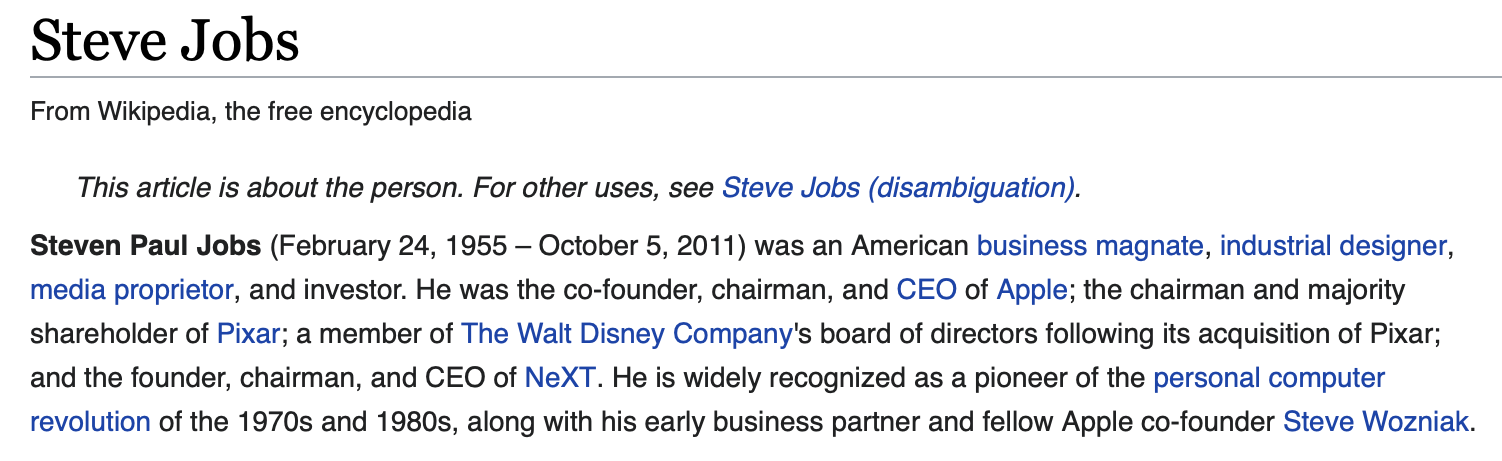
\includegraphics[width=\textwidth]{chapters/figures/SJ1.jpg}}
      \caption{A snippet from the Wikipedia article of Steve Jobs}
    \label{fig:wikisj}
  \end{minipage}
  \end{figure}
The Wikipedia article of an entity: \textit{Steve Jobs} comprises sentences that have other entities Figure \ref{fig:wikisj}. Each of these entities is linked to its own Wikipedia page. Given a sentence from the Wikipedia page of \textbf{Steve Jobs} (E1), {\fontfamily{pcr}\selectfont "the chairman and majority shareholder of \textbf{PIXAR}} (E2)". Both E1 and E2 have their respective Wikipedia pages, but that does not give us enough information to find where the entities appear together.

From the free-text KG we extract: (1) the sentences in E1’s Wikipedia page that mention E2, (2) the sentences in E2’s page that mention E1, and (3) the sentences (anywhere) that mention both E1 and E2 \cite{delft}. Figure \ref{fig:ftkg} shows a snippet from the constructed Free-Text Knowledge Graph.

\begin{figure}
    \centering
  \begin{minipage}[b]{0.7\textwidth}
    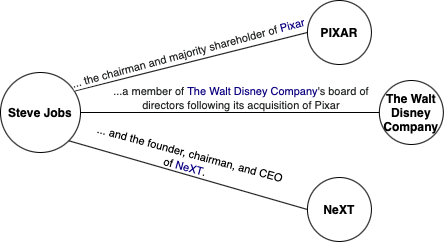
\includegraphics[width=10cm]{chapters/figures/KG1.jpg}
    \caption{A visual example of a Free-Text knowledge graph}
    \label{fig:ftkg}
    \end{minipage}
\end{figure}

\section{Indexing Free-Text KG}
Indexing is used to retrieve data from the database efficiently. Large data-dumps like Wikipedia have several lines of information mapped to various entities. Wikipedia has grown into one of the dominant knowledge sources of mankind, maintained by thousands of contributors \cite{dbpedia}. Indexing helps in querying the free-text knowledge graph to fetch the required results.
The indexed free-text KG has the following information:
\begin{itemize}
    \item \textbf{Page\_id}: An integer, the id of the Wikipedia page.
    \item \textbf{Title}: A string, the title of the Wikipedia page, usually an entity.
    \item \textbf{Text}: A string, sentence in the article that could have more than one entities.
    \item \textbf{Anchored\_Node}: The linked entities in the text. Linked entities refer to entities that have their own pages in Wikipedia. Every anchored\_node is represented as a key-value pair, where the key is the Wikipedia title of the anchored\_node and the value is the \textit{surface form} (the word as it appears in the text), of the anchored\_node. Consider the example sentence in the Wikipedia article of Steve Jobs, "\textit{In 2001, the original \textbf{Mac OS} was replaced with the completely new Mac OS X}". The entity \textit{Mac OS} is an anchored\_node which is represented as ["Classic Mac OS","Mac OS"]. The entity has its own Wikipedia article: \textit{Classic Mac OS} and occurs as \textit{Mac OS} in the Wikipedia article of Steve Jobs.
\end{itemize}
\begin{figure}
    \centering
    % \begin{minipage}[b]{0.7\textwidth}
    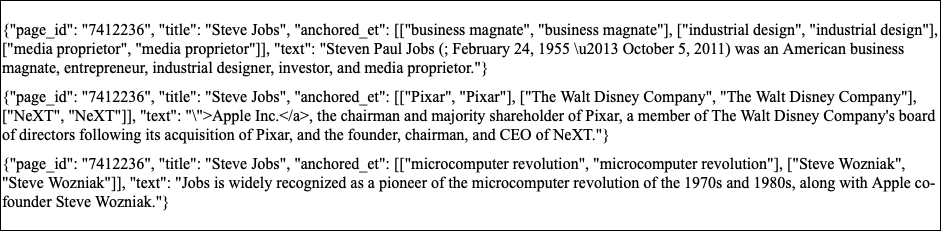
\includegraphics[width=0.8\textwidth,height=3cm]{chapters/figures/SJ2.jpg}
      \caption{Example sentences from the Free-Text Knowledge Graph}
    \label{fig:ftkgsent}
%   \end{minipage}
\end{figure}
Figure \ref{fig:ftkgsent} shows an indexed free text knowledge graph for a snippet of the Wikipedia page of Steve Jobs.

% \subsection{Searching the free-text KG}
The indexed free-text knowledge graph that is constructed has {\fontfamily{pcr}\selectfont 48,977,209} entries. Extracting information from this KG is an extensive task. We use Apache Solr\footnote{\label{solr}https://solr.apache.org/}, a highly scalable, robust, fault-tolerant open-source search platform, that enables easy integration with various programming languages \cite{solr}. Solr search \cite{lucene} manages to search through the index
based on the search string and returns relevant results. When a term is searched, the request handler is processed and then assigned to the query parser accordingly. The query parser validates the query for errors and then transforms it into an Apache Lucene’s Query\footnote{https://lucene.apache.org/core/} format based on the fields. Solr proved effective in our approach for fast retrieval of data due to its ability to achieve fast search responses as it searches using the index instead of the text. In Solr, a Document is the unit of search and index. An index contains one or more Documents, and a Document consists of one or more Fields. The documents of our data comprise of the \textbf{\textit{page\_id, title, anchored\_node}} and \textit{\textbf{text}} as the fields.

\textbf{Extended Knowledge Graph}: DBpedia is one of the most extensive knowledge graphs used in many Question Answering problems. Researchers prefer using DBpedia as it 
i) contains factual data from articles and infoboxes of the English Wikipedia Language Edition (WPLE), ii) is enriched with labels and abstracts from the largest Wikipedia Language Editions, iii) is enriched with links to external knowledge graphs and Web pages, iv) has a rich variety of classes of entities, v) contains approx. 900 million triples (Jan 2021) and is steadily growing. In the last three years, infoboxes in all WPLEs grew by 150\% and the English WPLE doubled in size. We use the DBpedia knowledge graph as it covers many domains\cite{dbpedia}. The DBpedia KG contains over 5.6 million entities and 111 million facts (consisting of subject-relation-object triples), which require over 14.2GB of storage space \cite{dbpedia}. Therefore, we sliced DBpedia and extracted all the relations and their corresponding subject-object pairs to create an extended KG. We boosted our indexed free-text KG with the information from the extended KG. These two separate KGs are used as the principal source of knowledge and act as the core of ReMLOFT.

\textbf{Relations from DBpedia}: \label{sec:relationsfromdbpedia} The relations from DBpedia were extracted from the latest DBpedia dump\footnote{https://www.dbpedia.org/resources/latest-core/}. The DBpedia dump consists of RDF triples represented as (subject,relation,object). Algorithm \ref{alg:sopextract}  explains the extraction of relations from the DBpedia dump.
We create a list of relations \textbf{R} which appends every unique relation encountered in the DBpedia triples (line 5).

\begin{singlespace}
\begin{algorithm}
\caption{Extracting subject,relation,object from DBpedia dump}\label{alg:sopextract}
 \hspace*{\algorithmicindent} \textbf{input}: Triples in the DBpedia dump, $<s,r,o>$ \\
 \hspace*{\algorithmicindent} \textbf{output}:  A hashmap whose key is a relation and value is a list of subject and object pairs, RMap
\begin{algorithmic}[1]
\State \textbf{R} = \{\}
\State RMap = hashmap $<$relation, list$<$(subject, object)$>>$
\For {\textbf{each} t in DBpedia triple }
\If {$t.r \notin \textbf{R}$}
    \State 	\textbf{R} = \textbf{R} $\cup$ t.r
    \State 	RMap[r] = {(t.s, t.o)}
\Else
\State 	RMap[r].add((t.s, t.o))
\EndIf
% \For {\textbf{each} t in DBpedia triple }
%     \State $\mathcal{R}_{DB}$ = $\mathcal{R}_{DB}$ $\cup$ r
%     \State $SO_{r}$= list(s,o)
\EndFor \\
\Return RMap
\end{algorithmic}
\end{algorithm}
\end{singlespace}

We only considered the relations that were of the  ontology/ (dbo:) or property/ (dbp:) types. Table \ref{tab:countrelations} shows the number of relations extracted from the DBpedia dump.
\begin{table}[H]
    \centering
    \begin{tabular}{|c|c|}
     \hline
     \textbf{Relations from DBpedia} & \textbf{Count} \\
    \hline
     ontology/ & 1437 \\
    \hline
    property/ & 52477 \\
    \hline
    \textbf{Total} & \textbf{53914} \\
    \hline
    \end{tabular}
    \caption{Number of relations in DBpedia}
    \label{tab:countrelations}
\end{table}

Some of the observations on the relations extracted from DBpedia's latest core that makes relation mapping more challenging are as follows:

\begin{enumerate}
\item Many relations occur in both the dbo: and dbp: namespace (850 relations). For example, \textit{dbo:spouse and dbp:spouse} are both valid relations in DBpedia. 

\item The DBpedia dump has relations with numerous spelling and captilization errors : \textit{dbp:date, dbp:Date, dbp:dAte, dbp:daTe, dbp:datE}, but they are considered as a single end url point in DBpedia.

\item Relations can be singular or plural. For instance, \textit{dbp:spouse, dbp:spouses}.

\item  The relations have special characters: punctuation marks (\textit{dbp:nextYear'sRace}), numbers (\textit{dbp:firstRider125Bike}), Greek Letters and characters from other languages apart from English.

% \item The dbp: or dbo: values could reference an rdf:type. RDF types are  used to state that an entity is an instance of a class. They do not define a relation, instead they point to an entity in DBpedia. For a natural language statement, \textit{"Proinsulin a protein"}, the triple is represented as 
% $<$Proinsulin,rdf:type,dbo:Protein$>$, 

\item Relations are concatenated strings in Camel case. For example, \textit{dbp:militaryRank and dbo:significantBuilding}.
\end{enumerate}

Hence, we filtered these relations by removing punctuation marks, Greek Letters, characters from other languages to make our process efficient. For relations that occur in both the dbo: and dbp: namespace, we consider them as one relation. For instance \textit{dbo:spouse} and \textit{dbp:spouse} is considered as one relation \textit{spouse}. We will refer to this list of filtered relations as $\mathcal{R}_{DB}$. $\mathcal{R}_{DB}$ represents the pool of all relations that make up our search space for the task of relation mapping.

\textbf{Subject-Object pairs from DBpedia}: Entities in DBpedia are connected by one or more relations. The entities are referred to as the subjects or objects connected using a relation. For every relation in \textbf{R} we can have various subject-object pairs. t.s, t.r and t.o represents the subject, relation and object in the DBpedia triple, respectively. We create a hashmap called RMap, whose key is the relation in the triple and value is a list of subject- object pairs. For every triple in DBpedia the list of subject-object pairs are extracted along with the relation. If a relation is unique, a new key is generated in RMap, otherwise, the subject-object pair is added to the list of the existing relation.
Figure \ref{fig:subject-object} shows a snapshot of some of the subject-object pairs for a relation dbo:largestCity, where the object (right) represent the largest city in the subject (left). The relation \textbf{dbo:largestCity} has 3247 subject-object pairs and \textbf{dbp:spouse} has 963 subject-object pairs.

\begin{figure}
    \centering
   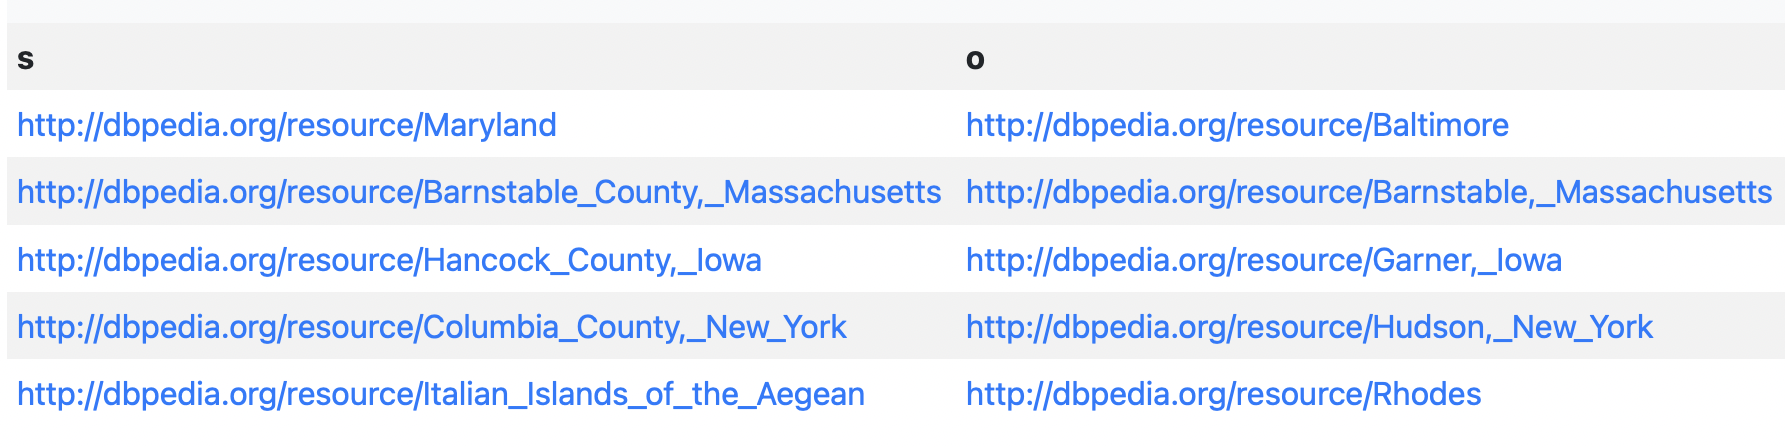
\includegraphics[width=15cm, height=4cm]{chapters/figures/subject-object.png}
    \caption{Snapshot of Subject-Object pairs for dbo:largestCity}
    \label{fig:subject-object}
\end{figure}

\subsection{Sentence Extraction}
Each relation in $\mathcal{R}_{DB}$ has numerous subject-object pairs. These subject-object pairs (anchored\_nodes) co-occur in sentences in the text corpus that we used, and are therefore stored in our free-text KG. Other approaches use linguistic resources such as Oxford dictionary\footnote{Oxford English Dictionary. 2nd ed. Oxford: Oxford University Press, 2004}, and semantic dictionaries like WordNet\cite{wordnet} to provide
synonyms, derived word forms, etc. The sentences extracted are a wealth of information as they contain the entities, their context and other lingual facts. We extract these shared sentences and utilize this information to extract words for relation labels.
\begin{singlespace}
\begin{algorithm}
\caption{Extracting sentences from FTKG}\label{alg:sentextract}
 \hspace*{\algorithmicindent} \textbf{input}: RMap, $\mathcal{R}_{DB}$ \\
 \hspace*{\algorithmicindent} \textbf{output}:  A hashmap whose key is a relation and value is the sentences retreived from FTKG, SMap
\begin{algorithmic}[1]
\State SMap = hashmap$<$relation, list$<$sentence$>>$
\For {\textbf{each} r in $\mathcal{R}_{DB}$}
\For {\textbf{each} (s,o) in RMap[r]}
    \State SMap[r].add(SELECT text from FTKG where s and o in title, anchored\_node, text)
\EndFor 
\EndFor \\
\Return SMap
\end{algorithmic}
\end{algorithm}
\end{singlespace}
Algorithm \ref{alg:sentextract} explains the process of extracting sentences for every relation r in $\mathcal{R}_{DB}$. The input to this algorithm is the hashmap RMap, which has the key as the relations and value as the list of subject-object pairs, obtained in Algorithm \ref{alg:sopextract} and the list of filtered relations $\mathcal{R}_{DB}$.
Each (s,o) pair in RMap is searched in the indexed free-text KG using Solr. Solr searches for the s and o in the title, anchored\_node and text fields of the free-text KG. The \textit{text} that contains both the s and o are added to SMap (line 4). 
The output of this algorithm is SMap which is a hashmap whose key is the relation and the value is the sentences obtained from the free-text KG for the subject-object pairs of that relation. 

A sample Solr query that searches the subject-object pair: Steve Jobs, Laurene Powell Jobs is as follows:
\begin{quote}
{\fontfamily{qcs}\selectfont select?fl=text\&q= \\
(text:"Steve Jobs" AND text:"Laurene Powell Jobs") OR \\
(title: "Steve Jobs" AND title:"Laurene Powell Jobs" ) OR \\
(anchored\_node:"Steve Jobs" AND anchored\_node:"Laurene Powell Jobs")}
\end{quote}
Here, fl represents the field \textit{text} to be returned and q represents the \textit{search entity} which is the subject and the object. 

The output of this algorithm is a hashmap whose key is the relation r, and value is a list of sentences represented by SMap. For each relation in $\mathcal{R}_{DB}$, we store the sentences that are extracted from the indexed free-text knowledge graph.

\subsection{Text Cleaning Pipeline}
\label{sec:TextCleaningPipeline}
Text Cleaning Pipeline comprises of a series of modules which is used to clean the sentences connecting the relation to its subject-object pairs.
Algorithm \ref{alg:dictcreation} shows how the extracted sentences in SMap (output of Algorithm \ref{alg:sentextract}) is used to create a dictionary of words for each relation in $\mathcal{R}_{DB}$. Figure \ref{fig:graphConstruct} explains the approach for an example relation \textbf{spouse}. 

\begin{singlespace}
\begin{algorithm}
 \hspace*{\algorithmicindent} \textbf{input}: SMap, $\mathcal{R}_{DB}$  \\
 \hspace*{\algorithmicindent} \textbf{output}: A hashmap of whose key is a relation and value is a list of (keyword, frequency) pairs, Dict
\begin{algorithmic}[1]
\caption{Text Cleaning Pipeline}\label{alg:dictcreation}
\State Dict = hashmap$<$relation, list$<$(keyword, frequency)$>>$
\For {each r in $\mathcal{R}_{DB}$}
\For {each s in SMap[r]}
    \State Text-Preprocessing(s) //Removes punctuation, links and numbers
    \State Tokenization and Stopword Removal(s) //splits the sentence into tokens and removes stopwords
    \State Lemmatization(s) //converts the tokens into lemma
    \State $List_{r}$ = clean keywords in s
    \State UpdateCount(Dict[r], $List_{r}$)
\EndFor
\EndFor
\State \textbf{return} Dict
\end{algorithmic}
\end{algorithm}
\end{singlespace}

\textbf{Text Pre-processing}: Text pre-processing plays a vital role in text mining. The first module under the Text Cleaning Pipeline is illustrated in Figure \ref{fig:graphConstruct}. This module removes the input text's links, HTML tags, numbers, and punctuation as these tokens do not add valuable information to our text (line 4). 

\textbf{Tokenization and Stopword Removal}: The next module creates tokens from the output of the Text Pre-processing module. 
We use the word\_tokenize() function from the NLTK\footnote{{\label{nltk}}https://www.nltk.org} library to break the sentences into possible tokens. The NLTK library also has a corpus of stopwords in various languages. The most common words in Wikipedia articles are pronouns, prepositions, articles etc., such as \textit{a, the, who, is, on, etc}. These words have negligible lexical content. 
We use the English language corpus to remove stopwords from these sentences. Removing stopwords reduces the extent of term space by reducing the total number of terms in the system, and hence, reducing the size and complexity of the system. Stopwords are removed from documents because those words are not considered as keywords in text mining applications\cite{porter_1980}.

\textbf{Lemmatization}: The final module in the Text Cleaning Pipeline converts the tokens to their lemmas (line 6). The lemma is the base form of the token. They can be obtained using rules based on part-of-speech tags, or lookup tables.\cite{spacy}. Modern lemmatization algorithms in comparison with stemming, provide higher quality lemmas\cite{9467919}. SpaCy is the current state-of-the-art technique that processes and interprets large volumes of text. Lemmatization using the SpaCy library as compared to NLTK\footnotemark[\ref{nltk}] is the most effective according to the quality criterion as they include the processing of endings such as \textit{-ed, - ing}, regardless of the publication topic\cite{9467919}. The recent upgrade of spaCy is more effective in POS (parts-of-speech) tags than their previous versions\cite{spacy}. 

For example, if the input text to the Text Cleaning Pipeline is, "{\fontfamily{pcr}\selectfont The first generation of iPod was released October 23, 2001.}", the output of the lemmatization module would be a list of five keywords {\fontfamily{pcr}\selectfont ["first", "generation", "ipod", "release", "october"]}.

\begin{figure}
    \centering
    \fbox{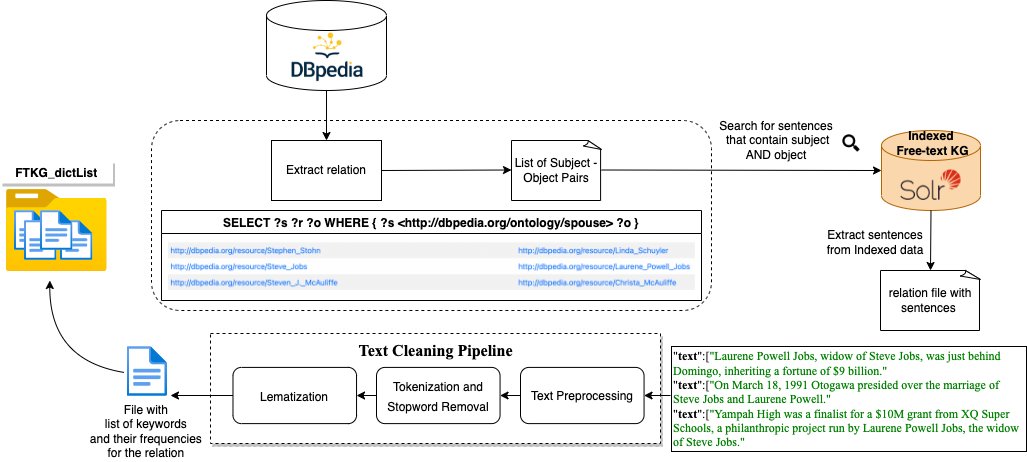
\includegraphics[width=15cm, height=7cm]{chapters/figures/GraphConstruct.png}}
    \caption{Dictionary Construction}
    \label{fig:graphConstruct}
\end{figure}

\textbf{Dictionary Creation}: The output of the Text Cleaning Pipeline is a list of keywords from the sentences in SMap (line 7). A dictionary is created from this list of keywords. We use a counter to tally the frequency of keyword occurrence in the file (line 8). The higher the count, more the keyword relates to the relation. We filter the top 100 keywords in each of these relation files. 

The total number of unique keywords obtained for each relation varies greatly. Some relations have keywords with a frequency of 100,000 while some relations have keywords with a frequency of 1. Relations that have keywords with frequencies in the order of thousands have a large number of unique keywords ($\sim$ 100 thousand words). In order to obtain a consistent parameter across all the relations with varying frequencies of occurrence, we choose the top 100 keywords. We found that the top 100 keywords contribute to the most associated words for a given relation as compared to using all the words in the relation files.

The output of Algorithm \ref{alg:dictcreation} is the dictionary Dict, which is also a hashmap whose key is the relation and value is a list of 100 keywords-number of occurrences pairs.

Using the example relation \textbf{spouse}, the top 3 keywords in the dictionary for \textbf{spouse}, Dict[spouse], are {\fontfamily{pcr}\selectfont
("marry", 93733), ("wife", 47744), ("daughter", 34588)
}.
\section{Using the Free-text KG}
{\label{usingfreetextkg}}
The relation list with the most common words along with their frequency of occurrence formulated from free-text KG, is the foundation knowledge graph of ReMLOFT, \textbf{Dict}. We will use the following question as a running example throughout this section, Q: {\fontfamily{pcr}\selectfont Which river does the Brooklyn Bridge cross?}.

\subsection{Pre-processing the Natural Language Question}
\label{sec:preprocessnlq}
The objective of this pre-processing is to extract the candidate keywords in the question that can be used to map to relations in the KG. This pre-processing includes (1) identifying entities in the question, (2) removing these entities, and (3) preparing the remaining keywords.

\textbf{Identifying Entities:} We first identify the entities in the question Q as the Question Entity Nodes, $E_{Q}=\{e_{i} | e_{i} \in Q \}$.  In Figure \ref{fig:approach}, the entity in the Question is \textbf{Brooklyn Bridge}. For a question with multiple entities: {\fontfamily{pcr}\selectfont In which films directed by Garry Marshall was Julia Roberts starring?}, the system identifies \textbf{Gary Marshall} and \textbf{Julia Roberts} as the entities. Several NER approaches can be used to identify the entities in the question \cite{falcon, falcon2}. 

\textbf{Removing Entities:} Once identified, the entities $E_{Q}$ are removed from the question. If the entity is a n-gram (n words), all the words occurring in the entity are removed from the question. In our example question, \textit{Brooklyn\_Bridge} is a bi-gram entity found in DBpedia, hence, the keywords Brooklyn and Bridge are removed from the question.

\begin{figure}[h]
    \centering
   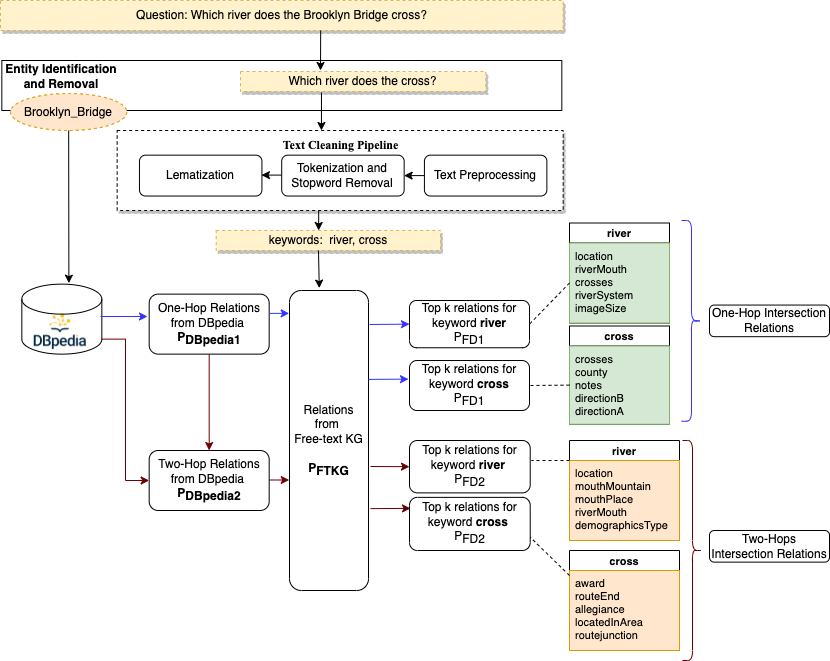
\includegraphics[width=15cm, height=10cm]{chapters/figures/Approach.png}
    \caption{Illustration of the steps of ReMLOFT using the example question "Which river does the Brooklyn Bridge cross?"}
    \label{fig:approach}
\end{figure}

\textbf{Preparing Remaining Keywords:} Once the entities $E_{Q}$ are removed from Q, the other keywords in Q are passed through the modules of the Text Cleaning Pipeline to obtain the lemmatized Keywords, $KW_{Q}=\{kw_{i} \; |\; kw_{i} \in Q \}$. The keywords first undergo Text pre-processing, where the punctuation, numbers and links are removed. They are then tokenized followed by the removal of stopwords. Finally, the keywords are lemmatized to their lemma which is the base form of the keyword. In our running example question, after the removal of the entities, \textit{"Which river does the cross?"}, are the remaining keywords in the question. After the processing the keywords, we get \textit{river} and \textit{cross} as the final keywords that we will use for relation mapping.

\subsection{Extracting candidate relations from DBpedia}
The objective of this step is to reduce the search space of relations from which we will map tokens in the questions to the relations. We do this by focusing on the set of entities $E_{Q}$ extracted from Q. These entities are queried in DBpedia to retrieve the relations associated with them. Algorithm \ref{alg:candidaterelations} shows the extraction of candidate relations from DBpedia. The input of Algorithm \ref{alg:candidaterelations} is the set of entities $E_{Q}$ extracted from Q. The output is a list of relations found one-hop or two-hops away from the entities in $E_{Q}$.

\begin{singlespace}
\begin{algorithm}
\caption{Extracting candidate relations from DBpedia}\label{alg:candidaterelations}
 \hspace*{\algorithmicindent} \textbf{input}: Entities from the Question, $E_{Q}$   \\
 \hspace*{\algorithmicindent} \textbf{output}: A list of candidate relations at one-hop and two-hops intersection
\begin{algorithmic}[1]
\For {\textbf{each} e in $E_{Q}$}
    \State $P_{DBpedia1}$= SELECT distinct ?r where \{?e ?r ?o UNION ?s ?r ?e\}
        \State Pre-process $P_{DBpedia1}$
    \For {\textbf{each} r in $P_{DBpedia1}$}
        \State $P_{DBpedia2}$=
        \State SELECT DISTINCT ?r where
        \State\{e ?r ?x. \{?x ?r ?o.\} UNION \{?s ?r ?x.\}\} AND 
        \State SELECT DISTINCT ?r where 
        \State \{?x r e.\{?x ?r ?o.\} UNION \{?s ?r ?x.\}\}
    \EndFor
    \State Filter unique /ontology \& /property relations
\EndFor
% \State $P_{DB}=P_{DBpedia1} \cup P_{DBpedia2}$
% \State \textbf{return} $P_{DB}, P_{DBpedia1}, P_{DBpedia2}$
\State \textbf{return} $P_{DBpedia1}, P_{DBpedia2}$
\end{algorithmic}
\end{algorithm}
\end{singlespace}


\textbf{First-Hop relations} $P_{DBpedia1}$: The relations that link an entity to its nearest neighbour (line 2). A given entity can be a subject or an object when connected using a relation. We find all the distinct relations that connect the entity to another entity in DBpedia.

\textbf{Second-Hop relations} $P_{DBpedia2}$: The relations that link the nearest neighbour to their neighbours (second-hop neighbour) (lines 5-9). 

\begin{figure}
    \centering
   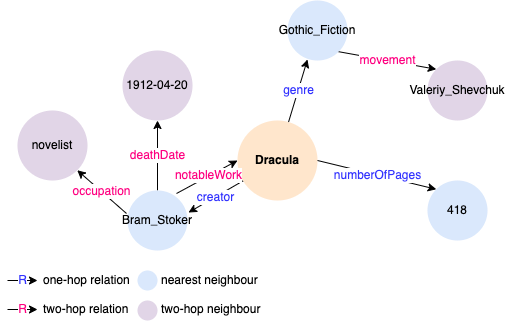
\includegraphics[width=12cm, height=8cm]{chapters/figures/Hop.png}
    \caption{The one-hop and two-hops relations and entities for dbr:Dracula}
    \label{fig:hop}
\end{figure}

We use the concept of two hops as some questions have answers in the second hop relations. While questions like our running example have the correct answer as one of the one-hop neighbouring entities, questions like {\fontfamily{pcr}\selectfont When did the creator of Dracula die?}, whose subgraph is shown in Figure \ref{fig:hop}, have the correct answer as one of the second-hop neighbouring entities. In the above example, the question has two keywords \textbf{creator} and \textbf{die} that should be mapped to the relations \textbf{creator} and \textbf{deathDate}, respectively. The relation \textbf{creator} is obtained one hop away from the entity, \textbf{Dracula}, identified in the question. However, the second relation \textbf{deathDate} is two-hops away from \textit{Dracula}. In order to retrieve \textbf{deathDate} we first traverse to the creator \textbf{Bram\_Stroker} and then to the deathDate of Bram\_Stroker, \textbf{1912-04-20}. 

We limit our approach to the second hop relations as the number of neighbours increase exponentially with the number of hops.  We use the entities as both the subject and the object while querying in Dbpedia, Algorithm 4 (line 6-9). 

Therefore, starting from the identified entities in the questions $E_{Q}$, we retrieve all the one-hop and two-hops away relations $P_{DBpedia1}$ and $P_{DBpedia2}$, respectively.

% A unique list of relations is obtained by combining the one-hop and two-hops away relations, $P_{DB}$ (line 13).
% \begin{equation}
%   P_{DB}=P_{DBpedia1}\cup P_{DBpedia2} 
% \end{equation}

\begin{singlespace}
\begin{algorithm}
 \hspace*{\algorithmicindent} \textbf{input}: Tokenized and Lemmatized keyword: key  \\
 \hspace*{\algorithmicindent} \textbf{output}: List of candidate relations from FTKG, $P_{FTKG}$
\begin{algorithmic}[1]
\caption{Extracting candidate relations from the Free-Text KG}\label{alg:extractFTKG}
\For {key in $KW_{Q}$}
\For {each entry in List(keyword, occurrencesNum)}
        \If {key == keyword}
            \State $P_{FTKG}$ = $P_{FTKG}$ $\cup$ (r,[key,occurencesNum])
        \EndIf
\EndFor
\EndFor
\State \textbf{return} $P_{FTKG}$
\end{algorithmic}
\end{algorithm}
\end{singlespace}

\subsection{Extracting Candidate Relations from the Free-text KG}
\label{sec:extractftkgrelations}
The question after the removal of the entity is left with a string of keywords $KW_{Q}$. For our running example question: the keywords obtained are $KW_{Q}$={\fontfamily{pcr}\selectfont river, cross}. Algorithm \ref{alg:extractFTKG} explains the steps for relation extraction from the Free-Text KG. Every keyword in $KW_{Q}$ (processed keywords) is searched in the all the dictionaries $Dict_{r}$, which is list of keywords and the number of occurrences of the keywords. If the search is successful, the \textit{relation} is concatenated with the keyword and number of occurrences which is represented as \textbf{(relation: [keyword, occurencesNum])} (line 4). The output of this extraction algorithm is a list of relations from the free-text KG, $P_{FTKG}$. We sort this list based on the \textbf{occurencesNum} of the keyword.

\subsection{Candidate List Generation}
\label{sec:candidatelist}
The output of the previous processes are the following sets of relations: 
\begin{enumerate}
    \item $P_{DBpedia1}$ (the one-hop relations from the entities identified in the question),
    \item $P_{DBpedia2}$ (the two-hops relations from the entities identified in the question), 
    \item $P_{FTKG}$ (the relations associated with sentences that include the keywords in the question).
\end{enumerate}
 In this final step, the objective is to generate the top-k candidate relations to display to the users to choose from. This is going to be based on the intersections of the aforementioned sets of relations as follows:

\textbf{One-Hop Intersection Relations, $P_{FD1}$} : This is the intersection of the one-hop relations from DBpedia, $P_{DBpedia1}$ and the relations obtained from the free-text KG, $P_{FTKG}$. This is sorted based on number of occurrences of the keyword in $P_{FTKG}$.
\begin{equation}
    P_{FD1}=P_{DBpedia1} \cap P_{FTKG}
\end{equation} 
% As shown in Figure \ref{fig:my_label}, for k=3, the keyword \textbf{river} matches {\fontfamily{pcr}\selectfont location, riverMouth and crosses} and the relation \textbf{cross} matches {\fontfamily{pcr}\selectfont crosses, country and notes}.
% \[P_{FD1}=P_{DBpedia1} \cap P_{FTKG}\]

\textbf{Two-Hops Intersection Relations, $P_{FD2}$} : This is the intersection of the two-hops relations from DBpedia, $P_{DBpedia2}$ and the relations obtained from the free-text KG, $P_{FTKG}$. This is sorted based on number of occurrences of the keyword in $P_{FTKG}$.
\begin{equation}
    P_{FD2}=P_{DBpedia2} \cap P_{FTKG}
\end{equation} 

% \textbf{Final Intersection, $P_{Final}$} : The relations obtained by combining the relations in the one-hop intersection relations and the two-hops intersection relations.
% \begin{equation}
%     P_{Final}=P_{FD1}+P_{FD2}
% \end{equation}

Figure \ref{fig:approach} shows the one-hop and two-hops intersection relations for our running example question where k=5 , based on the number of occurrences. The keyword \textbf{river} matches {\fontfamily{pcr}\selectfont location, riverMouth, crosses, directionB and directionA} and the relation \textbf{cross} matches {\fontfamily{pcr}\selectfont crosses, country, notes, riverSystem, imageSize} in the one-hop intersection. The keyword \textbf{river} matches {\fontfamily{pcr}\selectfont location, mouthMountain, mouthPlace, riverMouth and demographicsType} and the relation \textbf{cross} matches {\fontfamily{pcr}\selectfont award, routeEnd, allegience, locatedInArea and routeJunction} in the two-hops intersection.

\section{Interactive User Interface} 
We introduce an interactive user interface for ReMLOFT. This interface is shown in Figure \ref{fig:userinterface}. The user interface presents a text box for the user to type their natural language question. After the user clicks "\textbf{Recommended Relations}", the question is pre-processed using the steps discussed in Section \ref{sec:preprocessnlq}. The interface displays the processed keywords and the top-5 candidate relations extracted from the one-hop relations for each displayed keyword. In our running example, the user enters the question and we display the top-5 relations for the keywords \textit{river} and \textit{cross}.

% We propose a modified method where we display the best of the two results obtained from the One-Hop Intersection Relations, $P_{FD1}$ and Two-Hops Intersection Relations, $P_{FD2}$. This is effective for complex questions who have correct answers in the relations that are present two-hops away. 

In case the displayed relations do not satisfy the user's information needs, they can view an extended list pf candidate relations by clicking on "\textbf{View More Relations}". This would display the two-hops intersection relations for each keyword. 
\begin{figure}[h]
    \centering
    \fbox{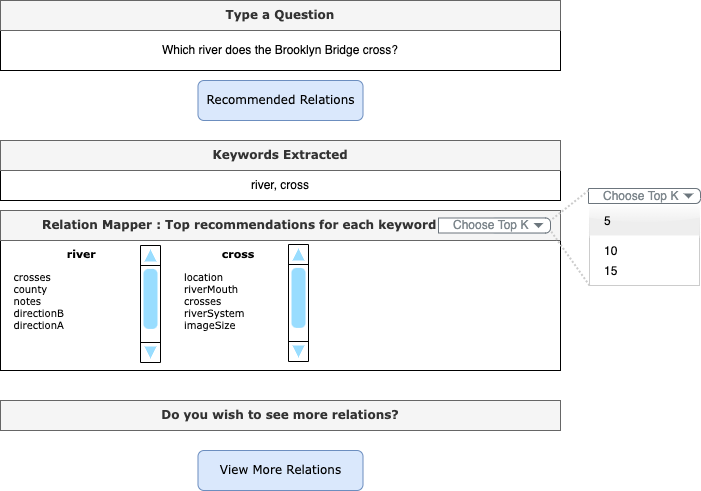
\includegraphics[width=\textwidth, height=11cm]{chapters/figures/interactive-2.png}}
    \caption{User Interface of ReMLOFT}
    \label{fig:userinterface}
\end{figure}
Given the typically large number of candidate relations obtained from the One-Hop Intersection Relations, $P_{FD1}$ and Two-Hops Intersection Relations, $P_{FD2}$ in a dataset, we limit the number of recommendations to top-5. We provide the user the flexibility to restrict or expand the top-k value from a drop-down. The idea is that the system assists the user to enhance query construction. 
The recommended relations help the user build superior SPARQL queries to retrieve answers to their questions over any knowledge graph. 

\end{sloppypar}